\documentclass[11pt,a4paper]{amsart}
%\documentclass[paper=a4, fontsize=11pt]{scrartcl}
%\documentclass[12pt, final]{sreport}
\usepackage[utf8]{inputenc}
\usepackage[icelandic]{babel}
\usepackage[T1]{fontenc}
\usepackage{color}
\usepackage{amsmath, amsthm, amssymb, amsfonts}
\usepackage{enumerate}
\usepackage{url}
\usepackage{cite}
\usepackage{listings}
\usepackage{graphicx}
\usepackage{fancyhdr}
\usepackage{booktabs}
\usepackage{float}
\usepackage{hyperref}
\usepackage{caption}
\usepackage{subcaption}
\usepackage{setspace} 
\usepackage{lipsum}
\usepackage{ifthen}
\usepackage{geometry}

%\onehalfspacing
%\addtolength{\textheight}{2.4cm}
%\addtolength{\hoffset}{-1.2cm}
%\addtolength{\voffset}{-2cm}
%\addtolength{\textwidth}{2.3cm}

% Define new commands and operators
\newcommand{\N}{\mathbb{N}}
\newcommand{\No}{\N_0}
\newcommand{\Z}{\mathbb{Z}}
\newcommand{\perms}{\mathfrak{S}}

\DeclareMathOperator{\prst}{\mathcal{P}} 
\DeclareMathOperator{\rem}{rem}	
\DeclareMathOperator{\id}{id}
% End of new commands definitions

% Setup theorem styles
\theoremstyle{plain}
\newtheorem{theorem}{Theorem}[section]
\newtheorem{proposition}[theorem]{Proposition}
\newtheorem{lemma}[theorem]{Lemma}
\newtheorem{corollary}[theorem]{Corollary}
\newtheorem{conjecture}[theorem]{Conjecture}

\theoremstyle{definition}
\newtheorem{definition}[theorem]{Definition}
\newtheorem{example}[theorem]{Example}

\theoremstyle{remark}
\newtheorem*{remark}{Remark}
% End of theorem styles setup



\begin{document}

%\title{Hópaverkefni 1 \\ Áhrif Iceland Airwaves á gistinætur}
%\authors{Arnar Ingi Halldórsson, Halldór Stefánsson, Hjörleifur G. Bergsteinsson, Lárus Ívar Ívarsson og Þór Tómasarson}
%\address{Reykjavik University,
%Menntavegi 1, \newline 101 \mbox{Reykjavík}, Iceland}
%\date{\today}
\newcommand{\HRule}{\rule{\linewidth}{0.5mm}}

\begin{titlepage}

\begin{center}
% Upper part of the page
%\includegraphics[width=0.55\textwidth]{rulogo.png}\\[4.0cm]    
%\includegraphics[width=4cm]{rulogo.png}

%\textsc{\LARGE Háskólinn í Reykjavík}\\[1.5cm]

\textsc{\LARGE Gagnavinnsla}\\[0.5cm]
\textsc{\Large Hópaverkefni 1}\\[0.6cm]

% Title
\HRule \\[0.4cm]
{ \Huge \bfseries Áhrif Iceland Airwaves á gistinætur á Íslandi}\\[0.2cm]

\HRule \\[1.5cm]


% Author and supervisor
\begin{minipage}{0.49\textwidth}
\begin{flushleft} \large
\emph{Nemandi:}\\
Arnar Ingi Halldórsson\\
Halldór Stefánsson\\
Hjörleifur G. Bergsteinsson\\
Lárus Ívar Ívarsson\\
Þór Tómasarson
\end{flushleft}
\end{minipage}
\begin{minipage}{0.49\textwidth}
\begin{flushright} \large
\emph{Kennari:} \\
Eyjólfur Ingi Ásgeirsson
\end{flushright}
\end{minipage}

\vfill

% Bottom of the page
{\large \today}



\end{center}

\end{titlepage}


Í þessu verkefni er okkur ætlað að skoða hvaða áhrif tónlistarhátíðin Iceland Airwaves hefur á gistinætur og gestakomur á hótelum og öðrum gististöðum, þar sem stuðst er við gögn frá Hagstofu Íslands sem gefa okkur gistinætur Íslendinga og útlendinga á Íslandi.\\

Við höfum hannað forrit með notendaviðmóti(mynd~\ref{fig:noten}) með það í huga að geta tekið inn vítt svið af gögnum. Gögnin þurfa að vera á ákveðinni uppsetningu. Til að keyra forritið þarf að keyra $ RunThisScript\_Main.py $. Sjá má $ csvReader.py $, þar sést hvernig uppsetningu gagna á að vera háttað. Það viðmót sem við höfum sett upp, er stillt upp fyrir tvær týpur af gagnauppsetningum, kallaðar 'Data Type 1' og 'Data Type 2'. Forritið er þannig uppsett að það aðlagar sig að gögnum sem sett eru inn hverju sinni, þ.e.a.s. hægt er að nota þetta forrit ár eftir ár. Hægt er að slá inn heiti á nýjum skrám í glugga notendaviðmótsins og ýta á þá hnappa sem í boði eru til að plotta og greina þau gögna sem valin eru.\par

Í myndum~\ref{fig:mynd2} og ~\ref{fig:mynd3} notum við aðferð minnstu kvaðrótar til þess að fá jöfnu bestu línu, til að hjálpa okkur að spá áframhaldinu. Jafnan fyrir íslenskar gistinætur er $$ y = 1077.9 \cdot x - 2139441.4  $$ og fyrir útlendinga $$ y = 4532.5 \cdot x - 9023834.1 $$
Okkar spá fyrir 2014 er þá að fjöldi gistinátta hjá íslendingum verður 31435 gistingar og hjá útlendingum 104650 gistingar.

Við sjáum á myndum~\ref{fig:mynd4} og ~\ref{fig:gist_spa} getum við lesið hvernig við teljum að október og nóvember hefðu þróast með Airwaves hjá Íslendingum og útlendingum miðað við raunþróun. Spáin fyrir október og nóvember er byggð á þróun gistinátta í september milli ára. Notast er við september vegna þess þar er enginn stórviðburður sem gæti haft áhrif á tölurnar. Hjá Íslendingum sjáum við að fjöldi gistinátta byrjar að aukast eftir 2003 miðað við spár bæði í október og nóvember og þar sem Airwaves var haldið í október fram að 2012, getum við ekki rekið þessa aukningar vegna Airwaves. Hjá útlendingum sjáum við einnig aukningu í október miðað við spá alveg aftur til 1999, sem hefur aukist jafn og þétt. Við getum gert ráð fyrir að Airwaves hafi áhrif á gistinætur útlendinga frá og með 2012, því þá er hátíðin haldin í nóvember og þar af leiðandi aukast gistingar augljóslega.

Út frá mynd~\ref{fig:gist_hlutf} sjáum að til ársins 2012 er lækkun á gistinóttum frá október til nóvember, en á þeim tíma var Airwaves í október. Árið 2012 og eftir það er Airwaves hins vegar haldið í nóvember og þá breytist hallatalan ekki eins mikið á milli október og nóvember.\par

Undanfarin ár hefur verið mikil aukning í ferðamönnum hér á landi eins og sést þegar gögnin eru skoðuð og því erfitt að meta hversu mikil áhrif Airwaves hefur á aukninguna. Þó teljum við um aukningu á gistinóttum sé að ræða vegna Airwaves og sést það aðallega á mynd~\ref{fig:gist_spa}, þegar hátíðin er haldin í nóvember og fjöldi gistinætra eykst augljóslega miðað við árin á undan.

\section{Viðauki}

\begin{figure}[H]
	\centering
	\begin{subfigure}[b]{0.4\textwidth}
		\includegraphics[height=40mm]{mynd2.png}
		\caption{$ Adferd\ minnsta\ kvadrarata $\label{fig:mynd2}}
	\end{subfigure}
	\begin{subfigure}[b]{0.4\textwidth}
		\includegraphics[height=40mm]{mynd3.png}
		\caption{$ Adferd\ minnsta\ kvadrarata $\label{fig:mynd3}}	
	\end{subfigure}
\end{figure}

\begin{figure}[H]
	\centering
	\begin{subfigure}[b]{0.45\textwidth}
		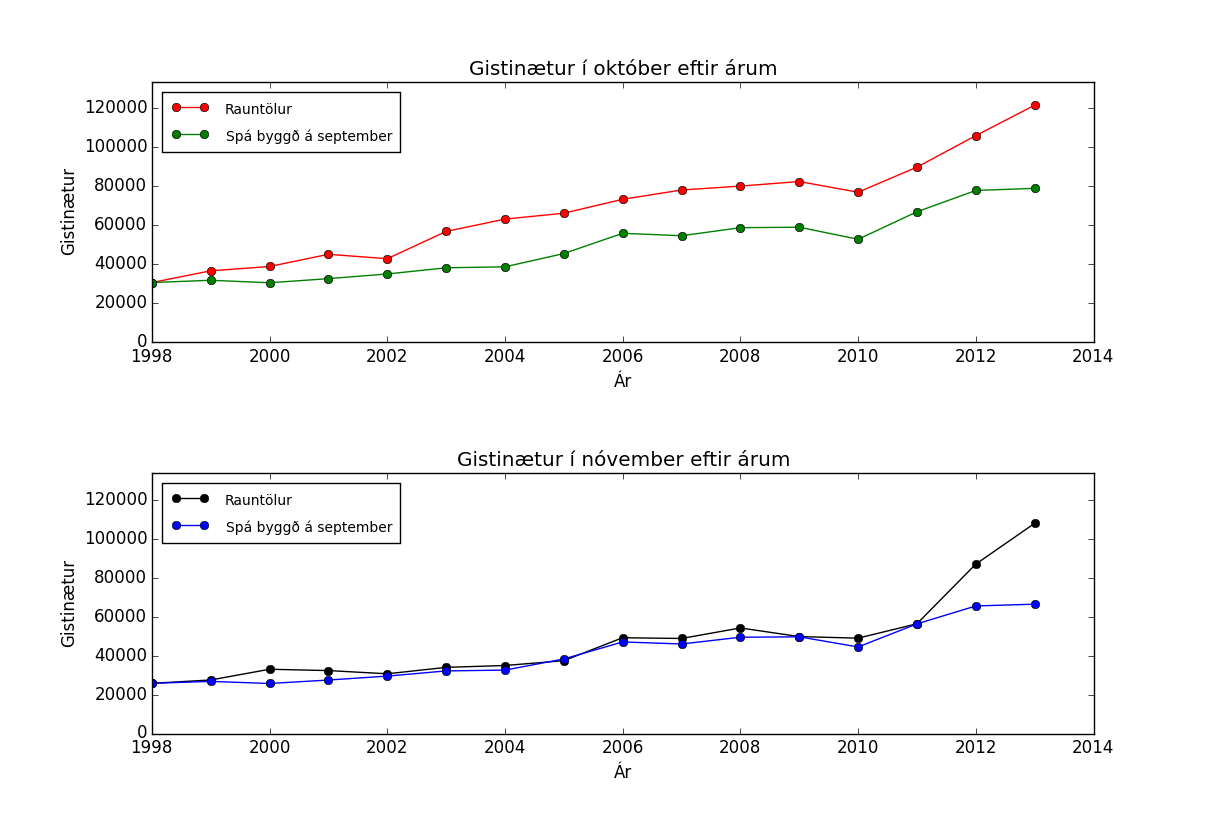
\includegraphics[height=40mm]{figure_3.png}
		\caption{$ Rauntolur\ og\ spar\ a\ gistinottum $\label{fig:mynd4}}
	\end{subfigure}
	\begin{subfigure}[b]{0.45\textwidth}
		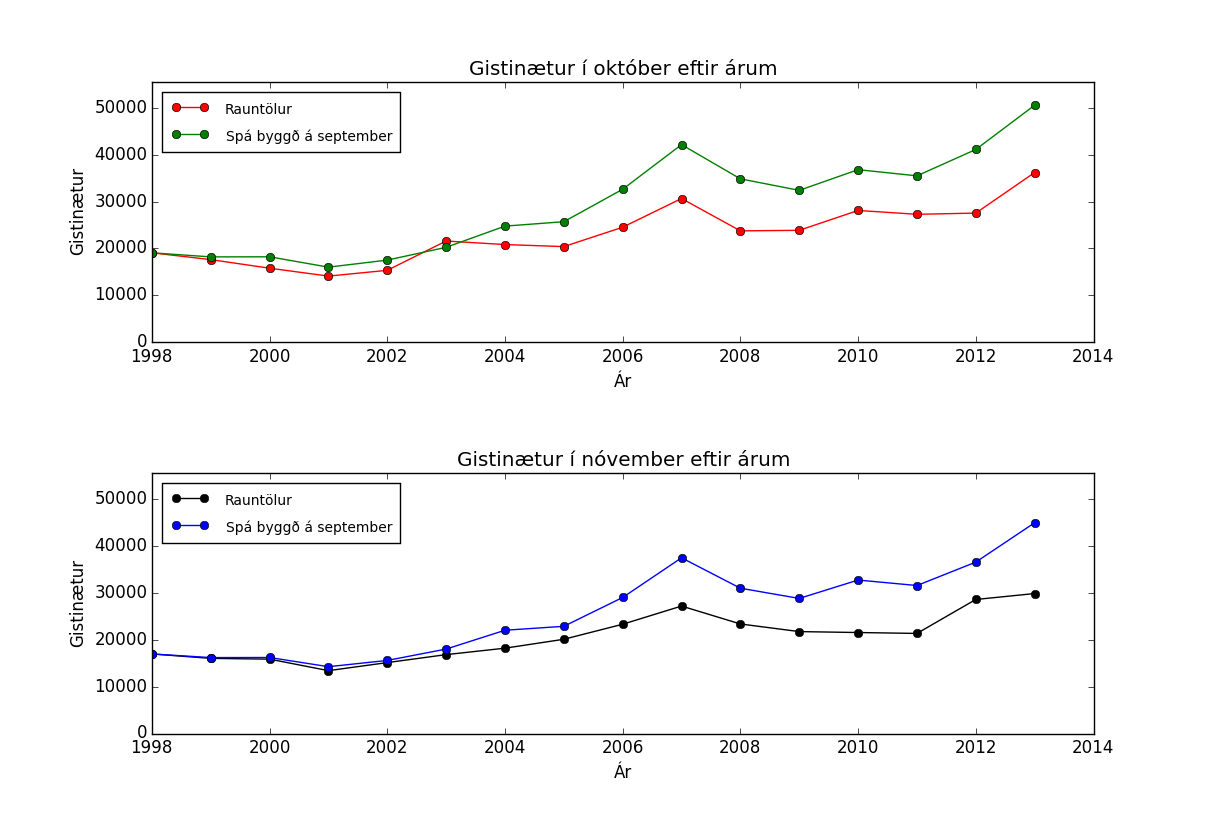
\includegraphics[height=40mm]{figure_2.png}
		\caption{$ Rauntolur\ og\ spar\ a\ gistinottum $\label{fig:gist_spa}}
	\end{subfigure}
\end{figure}

\begin{figure}[H]
\centering
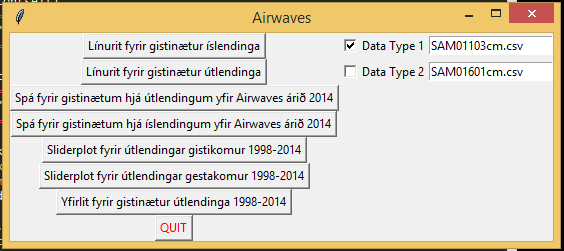
\includegraphics[height=30mm]{GUI.png}
\caption{$ Notendavidmot $\label{fig:noten}}
\end{figure}

\begin{figure}[H]
\centering
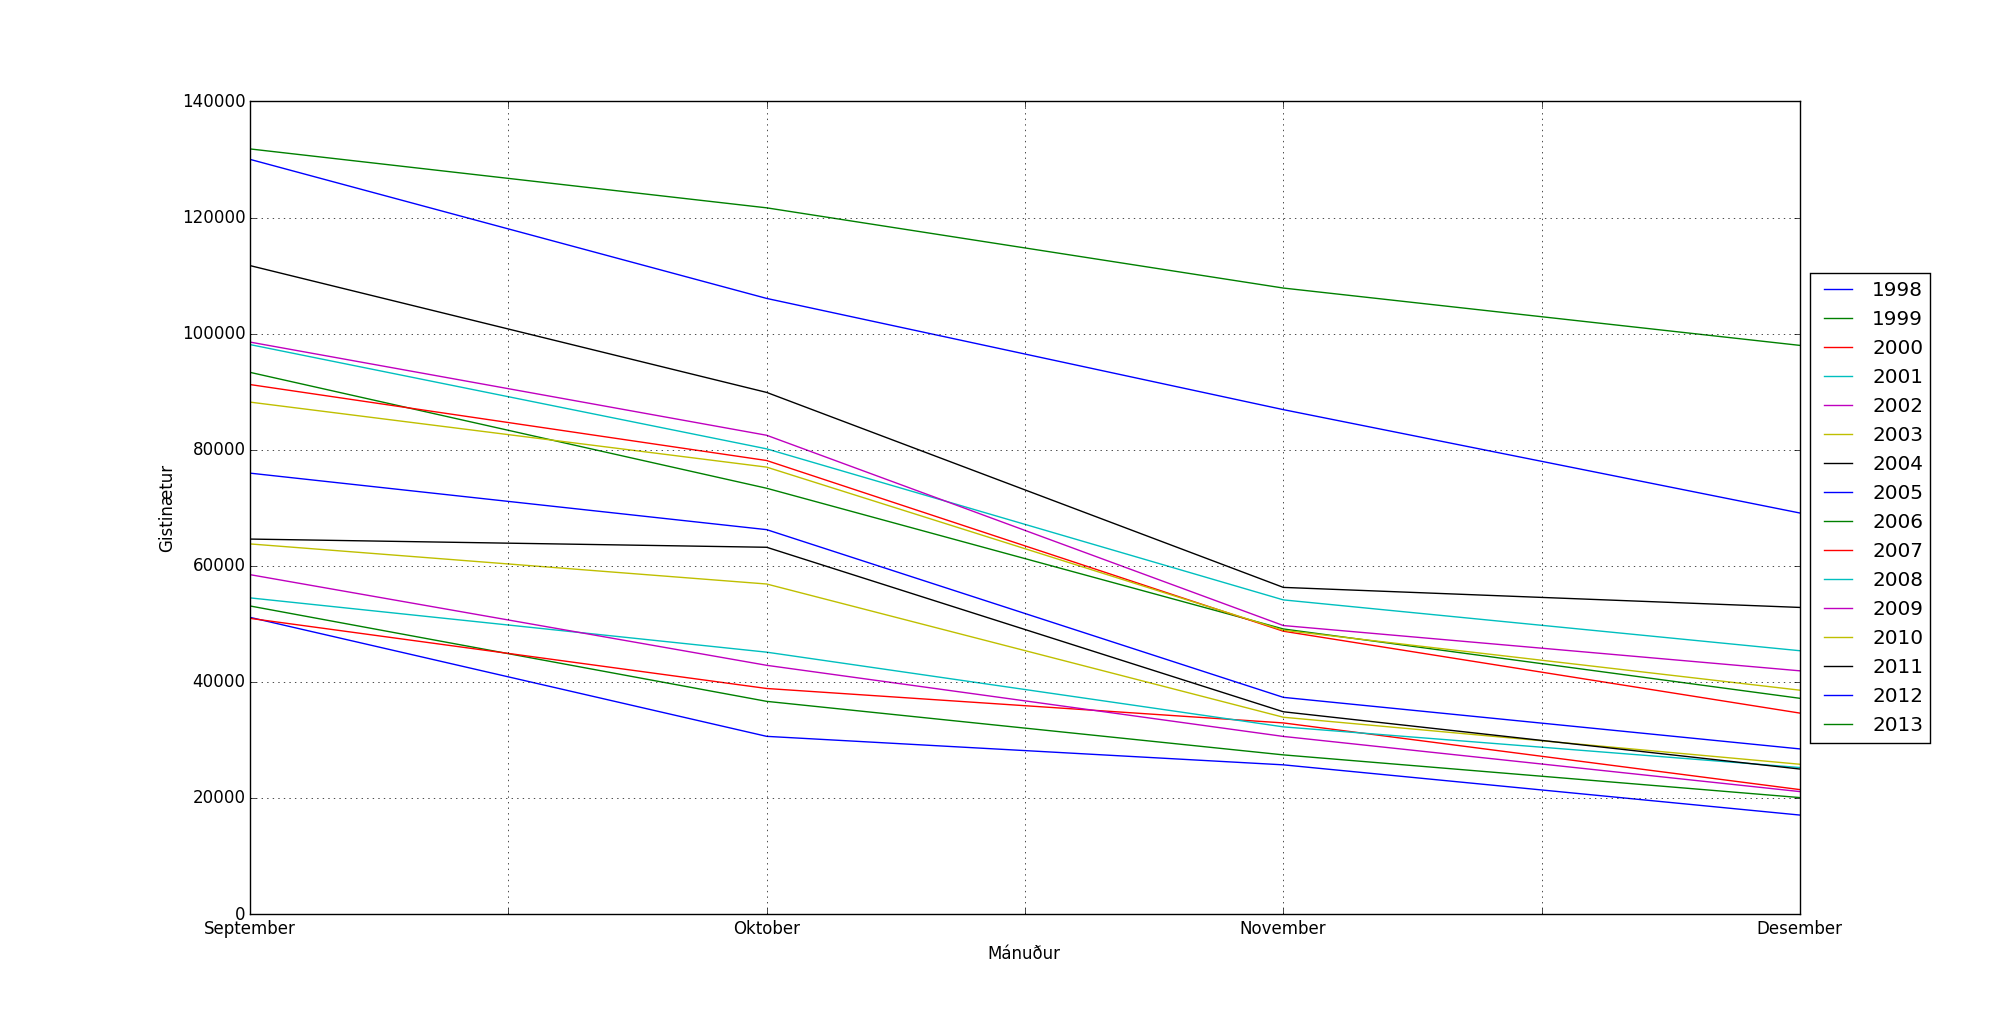
\includegraphics[height=40mm]{my_plot.png}
\caption{$ Gistinaetur\ manuda\ i\ kringum\ Iceland\ Airwaves $\label{fig:gist_hlutf}}
\end{figure}
	
\bibliography{citations}{}
\bibliographystyle{plain}
\end{document}